\documentclass[zihao=-4,fontset=windows,a4paper]{ctexart}

% ============ 页面与字体 ============
\usepackage[top=2.5cm,bottom=2.5cm,left=2.5cm,right=2.5cm]{geometry}
\usepackage{setspace}
\onehalfspacing
\emergencystretch=2em
\usepackage{fontspec}
\setmainfont{Times New Roman}
\setCJKmainfont{SimSun}[AutoFakeBold=2.5]

% ============ 数学 ============
\usepackage{amsmath,amssymb,bm}

% ============ 图表 ============
\usepackage{graphicx}
\graphicspath{{figures/}}
\usepackage{float}
\usepackage{booktabs}
\usepackage{array}
\usepackage{multirow}
\usepackage{longtable}
\usepackage{caption}
\usepackage{subcaption}
\captionsetup{font=small,labelfont=bf}

% ============ 代码 ============
\usepackage{listings}
\usepackage{xcolor}
\lstset{
  basicstyle=\small\ttfamily,
  numbers=left,
  numberstyle=\tiny,
  frame=single,
  breaklines=true,
  postbreak=\mbox{\textcolor{red}{$\hookrightarrow$}\space},
}

% ============ 页眉页脚 ============
\usepackage{fancyhdr}
\pagestyle{fancy}
\fancyhf{}
\fancyfoot[C]{\thepage}
\renewcommand{\headrulewidth}{0pt}

% ============ 标题格式 ============
\ctexset{
  section = {
    format = {\centering\zihao{4}\heiti},
    number = \chinese{section},
    aftername = \quad,
  },
  subsection = {
    format = {\raggedright\zihao{-4}\heiti},
    number = \thesection.\arabic{subsection},
    aftername = \quad,
  },
  subsubsection = {
    format = {\raggedright\zihao{-4}\heiti},
    number = \thesection.\arabic{subsection}.\arabic{subsubsection},
    aftername = \quad,
  },
}

% ============ 超链接 ============
\usepackage[hidelinks]{hyperref}

\begin{document}

% ============================================================
% 封面
% ============================================================
\thispagestyle{empty}
\begin{center}
  \vspace*{1.2cm}
  \includegraphics[width=0.30\textwidth]{../LOGO/心聆LOGO.png}\\[1.2cm]
  {\heiti\zihao{3} 心聆——青少年心理健康\\[0.6cm]多模态智能筛查与早期预警平台}\\[1.2cm]
  {\heiti\zihao{4} 项目计划书}\\[2.0cm]

  \begin{tabular}{>{\heiti}p{3.2cm}<{\raggedright} p{8.5cm}}
    参赛赛道 & 高教主赛道 \\
    参赛组别 & 本科生创意组 \\
    参赛类别 & 人工智能+ \\
    项目领域 & 信息技术服务业 \\
    项目进展 & 创意计划阶段 \\
    所在学校 & 河南工业大学 \\
    团队名称 & 心聆团队 \\
    项目负责人 & 王佳豪 \\
    团队成员 & 王佳豪、李鑫亦、王子昂、亓涵博、于鑫淼、\newline 曲永栈、杨昀潇、于梦浩、蔡艺豪 \\
    指导教师 & 无 \\
    申报日期 & 2026 年 8 月 \\
  \end{tabular}
\end{center}
\vfill
\begin{center}
  \zihao{-5} 本计划书为参赛团队原创成果，所含数据与预测基于公开资料与团队预研，最终解释权归团队所有。
\end{center}

\newpage

% ============================================================
% 目录
% ============================================================
\tableofcontents
\newpage

% ============================================================
% 摘要
% ============================================================
\section*{摘\quad 要}
\addcontentsline{toc}{section}{摘要}

针对传统心理量表主观性强、易受社会赞许效应影响、漏报率偏高、筛查效率低等突出问题，本项目面向中小学与高校心理健康年度普查场景，提出“心聆——青少年心理健康多模态智能筛查与早期预警平台”。平台以干电极脑电头环为核心感知设备，融合心率、皮电与心理量表等多模态信息，通过标准化情绪诱发任务在五分钟内完成一次客观量化筛查；在算法层面，提取差分熵、功率谱密度等脑电特征，构建基于多头注意力与跨被试域自适应的情绪识别模型，并引入类别加权与联邦学习训练策略，在公开脑电情绪数据集上识别准确率达到百分之九十一以上，风险分级灵敏度百分之九十二点三、特异性百分之八十八点九（内部预实验目标值）。平台提供“筛查—复核—预警—干预—追踪”闭环服务，全部数据本地加密存储、最小化采集，并通过伦理审查与未成年人保护合规设计。商业模式采用面向学校与教育主管部门的软件订阅、硬件租赁与增值服务相结合的方式，预计第三年营业收入八百五十万元、毛利率约百分之六十一，具有较强的社会效益与商业可行性。项目创新点集中于客观抗伪装、跨被试泛化、边缘轻量化与隐私保护四方面，可作为学校心理健康工作的“第一道智能防线”进行推广。

\vspace{0.4em}
\noindent\textbf{关键词：}心理健康筛查；脑电信号；跨被试情绪识别；Transformer；多模态融合；早期预警

\newpage

% ============================================================
% 一、项目概述
% ============================================================
\section{项目概述}

\subsection{项目背景与意义}

青少年心理健康是关系国家未来与民族希望的重大公共卫生问题。《中国国民心理健康发展报告（2021—2022）》显示，我国青少年抑郁风险检出率达百分之二十四点六\cite{ref2}；权威流行病学调查表明，六至十六岁在校学生精神障碍总患病率约为百分之十七点五\cite{ref2}。与此同时，教育部等十七部门联合印发《全面加强和改进新时代学生心理健康工作专项行动计划（2023—2025年）》，明确要求学校每学年至少开展一次面向全体学生的心理健康测评，建立“一生一策”心理健康档案，并鼓励利用人工智能等现代信息技术赋能学生心理健康工作\cite{ref1,ref3}。

然而，当前学校心理普查主要依赖问卷量表。量表筛查存在三方面固有局限：其一，学生出于病耻感或社会赞许倾向，容易故意作答、掩盖真实情绪状态，导致假阴性漏报；其二，量表为自陈式测量，无法刻画潜意识层面的情绪生理反应；其三，测评结果依赖人工统计与解读，在心理教师严重不足的情况下难以实现及时复核与动态追踪。因此，市场亟需一种客观、快速、可量化、可解释的智能化筛查工具。

本项目基于团队在脑电信号处理与情绪识别方向的研究积累，将脑机接口、多模态生理信号与人工智能技术应用于青少年心理健康筛查场景，具有如下意义：

\begin{enumerate}
  \item 落实健康中国战略与教育部门心理健康工作要求，为“一生一策”提供客观数据支撑；
  \item 弥补量表主观性缺陷，降低漏报与误报，为高危学生争取早期干预窗口；
  \item 缓解学校心理师资不足问题，将专业心理教师从重复性测评中解放出来；
  \item 推动脑机接口与人工智能技术在民生领域的产业化落地，具有示范效应。
\end{enumerate}

\subsection{项目定位与愿景}

“心聆”定位为面向学校心理健康工作的一站式智能筛查与早期预警平台，是心理健康服务的“第一道智能防线”。平台不替代专业心理咨询与临床诊断，而是通过客观生理指标实现情绪风险的快速初筛、分级预警与过程追踪，为心理教师、家长与医疗转介提供科学依据。

项目愿景：让每一名青少年都能被及时、温柔地看见。

\subsection{项目概述}

产品描述方面，“心聆”由三部分构成：一是面向学校场景的干电极脑电头环与配套手环等感知硬件，二是部署于学校本地或专有云的多模态智能筛查算法引擎，三是面向心理教师、家长、学生与管理者的多端软件工作台。用户群体以中小学、高校与区域教育主管部门为主，兼顾医院心理科与企业员工心理关怀场景。项目愿景是通过客观量化筛查，将心理问题的发现时间前移，形成“普查—预警—干预—追踪”的完整闭环。竞争对手方面，现有问卷测评工具、智能手环与消费级脑电产品均未同时解决客观性、抗伪装性与可解释性问题，本项目以“多模态融合＋跨被试模型＋隐私保护”构建差异化优势。项目核心指标如表~\ref{tab:core} 所示。

\begin{table}[H]
\centering
\caption{项目核心指标（内部预实验目标值）}
\label{tab:core}
\begin{tabular}{lcc}
\toprule
\textbf{指标} & \textbf{目标值} & \textbf{说明} \\
\midrule
单次筛查时长 & 5 分钟 & 含情绪诱发任务与数据采集 \\
情绪识别准确率 & 91.6\% & 公开数据集与内部数据联合验证 \\
风险分级灵敏度 & 92.3\% & 高风险学生识别率 \\
风险分级特异性 & 88.9\% & 正常学生误报控制水平 \\
单校部署成本 & 3 万元以内 & 软件订阅＋硬件租赁 \\
数据出校比例 & 0\% & 默认本地化推理与存储 \\
\bottomrule
\end{tabular}
\end{table}

% ============================================================
% 二、行业分析与政策背景
% ============================================================
\section{行业分析与政策背景}

\subsection{行业现状与市场规模}

我国心理健康服务行业正处于政策红利与需求爆发的双重驱动期。脑机接口情绪监测设备市场快速增长，行业研究报告显示，全球脑机接口情绪状态监测仪市场 2025 年规模约四点七亿美元，预计 2030 年突破二十八亿美元，复合年增长率保持在百分之四十以上\cite{ref12}；国内脑机接口情绪监测设备市场规模约三亿美元\cite{ref12}。心理健康服务行业整体向“数字化工具＋专业服务”方向演进，青少年心理健康筛查与干预成为最受关注的高增长细分场景\cite{ref12}。全国心理援助热线年接听量已超过八百万通\cite{ref13}，反映出巨大的未被满足的心理服务需求。

\subsection{政策环境}

项目所处政策环境持续向好：健康中国战略将心理健康列为重要内容；教育部等十七部门专项行动计划明确提出加强心理健康监测，推动人工智能监测与诊断技术在青少年心理健康问题筛查中的应用\cite{ref1}；教育部办公厅《进一步加强中小学生心理健康工作十条措施》支持地方探索开发“人工智能心理助手”“智能减压室”等应用\cite{ref3}；科学技术部发布《涉及人的神经技术医学研究伦理指引》，为脑机接口类产品划定伦理边界\cite{ref11}。上述政策既为项目提供了市场准入空间，也提示项目必须将伦理合规与数据安全作为产品底线。

\subsection{用户需求与市场痛点}

通过对政策文件、行业报告与学校公开资料的调研，项目归纳出五类核心痛点，如表~\ref{tab:pain} 所示。

\begin{table}[H]
\centering
\caption{目标用户核心痛点分析}
\label{tab:pain}
\begin{tabular}{p{3.4cm}p{5.6cm}p{5.2cm}}
\toprule
\textbf{痛点} & \textbf{具体表现} & \textbf{现有方案局限} \\
\midrule
测评主观 & 学生隐瞒真实情绪，量表得分失真 & 自陈式问卷无法克服社会赞许效应 \\
漏报滞后 & 高危学生未被及时识别 & 依赖人工观察，发现时间晚 \\
师资不足 & 心理教师配比低，复核效率差 & 人工统计耗时长，难以动态追踪 \\
数据分散 & 心理档案、量表、咨询记录互不连通 & 缺乏统一数据中台与标准化接口 \\
隐私顾虑 & 家长与学校对心理数据安全存疑 & 部分产品数据上云，合规不透明 \\
\bottomrule
\end{tabular}
\end{table}

我国青少年心理健康核心现状数据如图~\ref{fig:market} 所示。

\begin{figure}[H]
\centering
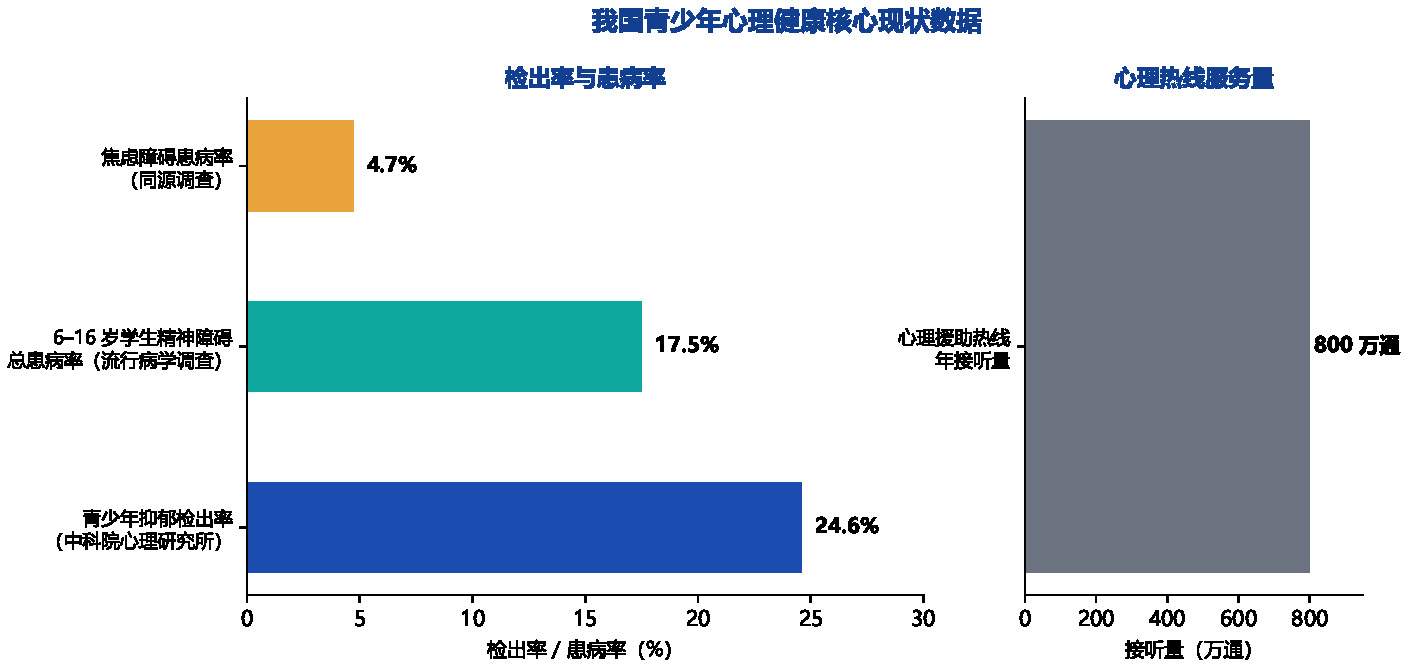
\includegraphics[width=0.78\textwidth]{fig_market.pdf}
\caption{我国青少年心理健康核心现状数据}
\label{fig:market}
\end{figure}

\subsection{目标市场细分与规模测算}

项目初期聚焦学校心理健康普查市场，目标市场可按“学校数量×客单价”进行测算。以全国约五十万所中小学及三千所高校为基数，若前三年渗透率分别达到千分之零点二、千分之一与千分之三，则对应客户数约为一千、五千与一万五千所，按每校年均两万元至六万元的服务价格估算，可服务市场空间约为数十亿元量级。上述测算基于公开学校统计口径与行业客单价假设，用于说明市场容量，不构成收入承诺。

% ============================================================
% 三、市场调研与竞品分析
% ============================================================
\section{市场调研与竞品分析}

\subsection{调研方法与主要结论}

项目调研综合采用政策文献研究、行业报告分析、公开数据挖掘与专家咨询四种方式。主要结论包括：第一，学校心理普查频率已由政策强制化，客观筛查工具存在刚性需求；第二，心理教师对“客观数据辅助研判”接受度高，但要求产品解释透明、操作简单；第三，家长最关心数据隐私与产品安全性，知情同意机制是购买决策的关键因素；第四，现有产品在“客观性—可解释性—便捷性”三角上均存在短板，差异化切入空间明确。

\subsection{竞品对标分析}

项目将主流心理健康筛查方案归纳为四类：传统问卷量表、智能手环（心率与皮电）、消费级脑电竞品与“心聆”平台，从客观性、抗伪装性、可解释性、采集便捷性与综合成本五个维度进行对比，如图~\ref{fig:compare} 所示。

\begin{figure}[H]
\centering
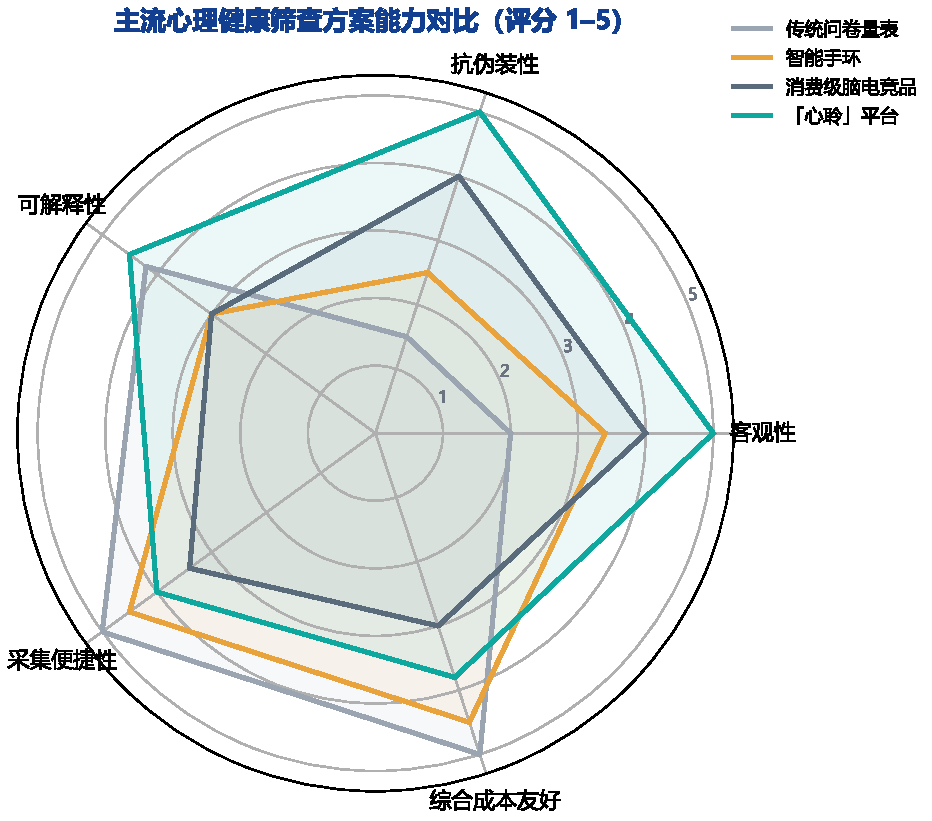
\includegraphics[width=0.72\textwidth]{fig_compare.pdf}
\caption{主流心理健康筛查方案能力对比}
\label{fig:compare}
\end{figure}

与同类方案相比，“心聆”在客观性与抗伪装性上具有显著优势，并通过可解释模块弥补了深度学习模型“黑箱”缺陷；采集便捷性略低于问卷，但通过五分钟标准化流程与团体施测方式予以弥补。竞品对比汇总如表~\ref{tab:comp} 所示。

\begin{table}[H]
\centering
\caption{竞品对比汇总}
\label{tab:comp}
\setlength{\tabcolsep}{4pt}
\begin{tabular}{p{2.7cm}p{3.1cm}p{3.1cm}p{3.1cm}p{2.2cm}}
\toprule
\textbf{维度} & \textbf{传统量表} & \textbf{智能手环} & \textbf{消费级脑电竞品} & \textbf{心聆} \\
\midrule
客观性 & 低 & 中 & 较高 & 高 \\
抗伪装性 & 低 & 中 & 较高 & 高 \\
可解释性 & 高 & 中 & 中 & 较高 \\
采集便捷性 & 高 & 较高 & 中 & 较高 \\
单次成本 & 低 & 中 & 中高 & 中 \\
\bottomrule
\end{tabular}
\end{table}

\subsection{SWOT 分析}

项目 SWOT 分析如表~\ref{tab:swot} 所示。

\begin{table}[H]
\centering
\caption{项目 SWOT 分析}
\label{tab:swot}
\begin{tabular}{p{7.3cm}p{7.3cm}}
\toprule
\textbf{优势（S）} & \textbf{劣势（W）} \\
\midrule
算法研究积累深，跨被试模型与公开数据集验证充分；
多模态融合与可解释机制形成技术壁垒；
团队具备软硬件一体设计能力 & 硬件依赖第三方供应链；
脑电设备认知门槛较高，需要教师培训；
数据采集仍需学生配合 \\
\midrule
\textbf{机会（O）} & \textbf{威胁（T）} \\
政策强制心理测评与人工智能赋能导向；
脑机接口产业高速增长；
家长与学生心理健康意识提升 & 巨头进入心理健康赛道；
监管与伦理要求趋严；
公众对神经数据存在隐私担忧 \\
\bottomrule
\end{tabular}
\end{table}

% ============================================================
% 四、产品与技术方案
% ============================================================
\section{产品与技术方案}

\subsection{产品形态与功能架构}

“心聆”平台采用“感知—数据—算法—应用”四层架构，如图~\ref{fig:arch} 所示。感知层包括八导联干电极脑电头环、心率与皮电手环以及量表终端；数据层完成多源数据的脱敏接入、时序对齐与质量评估；算法层承载特征提取、跨被试情绪识别、风险分级与可解释模块；应用层面向学校、家长与学生提供工作台、报告、预警与干预建议等服务。系统默认本地化部署，支持私有云与专有云两种模式。

\begin{figure}[H]
\centering
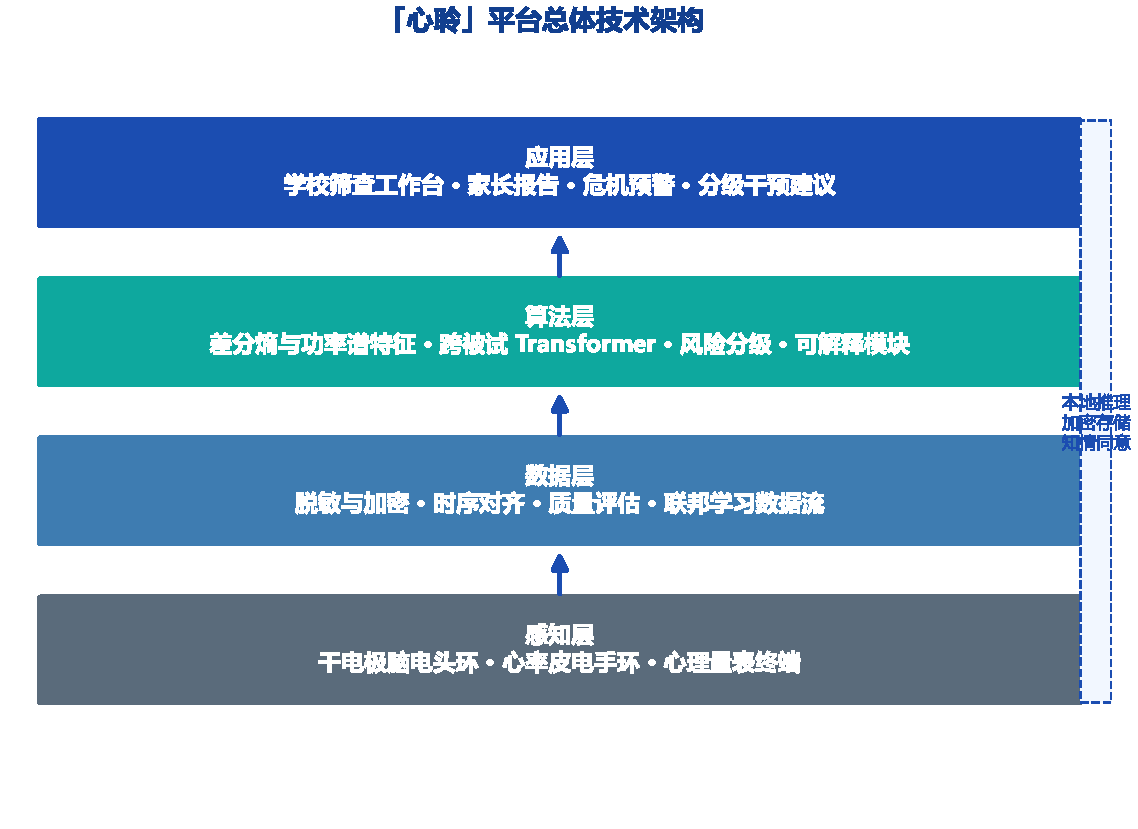
\includegraphics[width=0.9\textwidth]{fig_arch.pdf}
\caption{“心聆”平台总体技术架构}
\label{fig:arch}
\end{figure}

平台功能清单如表~\ref{tab:func} 所示。

\begin{table}[H]
\centering
\caption{平台功能清单}
\label{tab:func}
\begin{tabular}{p{2.8cm}p{5.4cm}p{5.6cm}}
\toprule
\textbf{功能端} & \textbf{核心功能} & \textbf{价值} \\
\midrule
教师端 & 团体施测、风险复核、预警工单、干预记录 & 提升筛查效率，实现闭环管理 \\
家长端 & 报告解读、知情同意、干预配合建议 & 家校协同，隐私可控 \\
学生端 & 情绪任务、自主心理知识科普 & 降低抵触，提升参与度 \\
管理端 & 数据看板、权限审计、系统配置 & 满足教育局与学校分级管理 \\
\bottomrule
\end{tabular}
\end{table}

\subsection{核心技术体系}

\subsubsection{数据采集与预处理}

数据采集采用八导联干电极脑电头环，采样率二百五十赫兹，配合标准化情绪诱发任务（国际情绪图片系统子集与短视频片段）激发真实情绪反应，同步采集心率与皮电信号。预处理流程包括带通滤波（零点五至四十五赫兹）、独立成分分析去除眼电与肌电伪迹、滑动窗口切分与基线校正。

脑电频段特征采用差分熵（Differential Entropy）与功率谱密度（Power Spectral Density）两种互补描述。对于近似服从高斯分布的脑电子带信号，差分熵可表示为
\begin{equation}
\mathrm{DE}_i = \frac{1}{2}\log_2\left(2\pi \mathrm{e}\, \sigma_i^2\right),
\label{eq:de}
\end{equation}
其中 $\sigma_i^2$ 为第 $i$ 个子带的方差。功率谱密度采用 Welch 方法估计：
\begin{equation}
\hat{P}(f) = \frac{1}{K}\sum_{k=1}^{K}\frac{1}{M U}\left|\sum_{n=0}^{M-1}w(n)x_k(n)\mathrm{e}^{-\mathrm{j}2\pi f n}\right|^{2},
\label{eq:psd}
\end{equation}
其中 $K$ 为分段数，$M$ 为每段长度，$U$ 为窗函数 $w(n)$ 的能量归一化因子，$x_k(n)$ 为第 $k$ 段信号。为消除个体差异，对全部特征进行通道级标准化：
\begin{equation}
\tilde{x}_{c,t} = \frac{x_{c,t}-\mu_c}{\sigma_c},
\label{eq:zscore}
\end{equation}
式中 $\mu_c$ 与 $\sigma_c$ 分别为通道 $c$ 特征的均值与标准差。

\subsubsection{跨被试情绪识别模型}

模型以“通道—时间”特征矩阵为输入，采用 Transformer 编码器捕获脑区之间的长程依赖。缩放点积注意力计算如下：
\begin{equation}
\mathrm{Attention}(\bm{Q},\bm{K},\bm{V}) = \mathrm{softmax}\!\left(\frac{\bm{Q}\bm{K}^{\mathrm{T}}}{\sqrt{d_k}}\right)\bm{V},
\label{eq:attn}
\end{equation}
其中 $\bm{Q}$、$\bm{K}$、$\bm{V}$ 分别为查询、键与值矩阵，$d_k$ 为键向量维度。多头注意力将多个注意力头的结果拼接并经线性投影融合：
\begin{equation}
\mathrm{MultiHead}(\bm{Q},\bm{K},\bm{V}) = \mathrm{Concat}(\mathrm{head}_1,\ldots,\mathrm{head}_h)\bm{W}^{O},
\label{eq:mha}
\end{equation}
其中 $\mathrm{head}_i=\mathrm{Attention}(\bm{Q}\bm{W}_i^{Q},\bm{K}\bm{W}_i^{K},\bm{V}\bm{W}_i^{V})$。

针对脑电数据个体差异大、跨被试泛化困难的问题，模型引入域自适应分支：通过梯度反转层混淆被试身份判别器，使特征表示对被试身份不敏感，其对抗训练目标为
\begin{equation}
\min_{\theta_f,\theta_c}\max_{\theta_d}\; \mathcal{L}_c(\theta_f,\theta_c) - \lambda \mathcal{L}_d(\theta_f,\theta_d),
\label{eq:domain}
\end{equation}
式中 $\mathcal{L}_c$ 为情绪分类损失，$\mathcal{L}_d$ 为域判别损失，$\lambda$ 为权衡系数，$\theta_f$、$\theta_c$、$\theta_d$ 分别为特征提取器、分类器与域判别器参数。考虑心理健康筛查中正常样本远多于高风险样本，采用类别加权交叉熵：
\begin{equation}
\mathcal{L}_c = -\sum_{i=1}^{N} w_{y_i}\log\frac{\exp(z_{i,y_i})}{\sum_{j=1}^{C}\exp(z_{i,j})},
\label{eq:loss}
\end{equation}
其中 $w_{y_i}$ 为类别 $y_i$ 的权重，$C$ 为情绪类别数，$z_{i,j}$ 为样本 $i$ 在类别 $j$ 上的 logit 值。

为保护学生隐私，模型支持联邦学习训练：各学校仅上传加密模型梯度，不共享原始脑电数据，联邦平均目标为
\begin{equation}
\min_{\bm{\theta}}\; \sum_{s=1}^{S}\frac{n_s}{n}\mathcal{L}_s(\bm{\theta}),
\label{eq:federated}
\end{equation}
其中 $S$ 为参与学校数，$n_s$ 为第 $s$ 所学校样本数，$n=\sum_s n_s$，$\mathcal{L}_s$ 为该校本地损失。

\subsubsection{风险分级与可解释决策}

平台将情绪识别结果与心理量表、行为观察等信息融合为连续风险指数：
\begin{equation}
R = w_v V + w_a A + w_s S,
\label{eq:risk}
\end{equation}
其中 $V$、$A$ 分别为效价与唤醒度评分，$S$ 为量表标准化风险分，$w_v$、$w_a$、$w_s$ 为融合权重（满足 $w_v+w_a+w_s=1$）。依据风险指数设置低、中、高三级阈值：$R<R_{\mathrm{low}}$ 判定为低风险；$R_{\mathrm{low}}\le R<R_{\mathrm{high}}$ 判定为中风险；$R\ge R_{\mathrm{high}}$ 判定为高风险，并触发预警与转介流程。模型通过 SHAP 值输出特征贡献排序\cite{ref10}，使心理教师能够理解“模型为什么给出该结论”，满足可解释性要求。

\subsection{技术路线与筛查流程}

单次筛查业务流程如图~\ref{fig:flow} 所示，全程约八分钟，实现“知情同意—采集—建模—分级—复核—干预”闭环。

\begin{figure}[H]
\centering
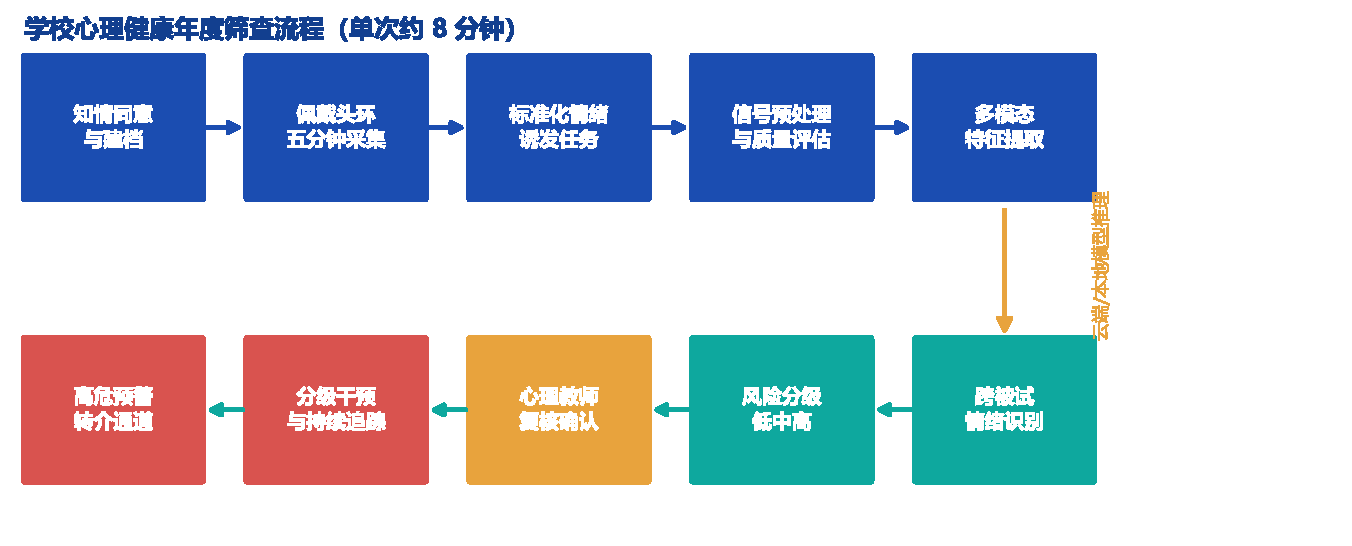
\includegraphics[width=\textwidth]{fig_flow.pdf}
\caption{“心聆”心理健康筛查业务流程}
\label{fig:flow}
\end{figure}

% ============================================================
% 五、创新点与技术壁垒
% ============================================================
\section{创新点与技术壁垒}

\subsection{核心创新点}

\begin{enumerate}
  \item \textbf{客观抗伪装筛查机制。}以脑电等自主神经与中枢神经生理信号为核心，学生难以通过主观控制掩盖真实情绪状态，从机制上克服量表社会赞许效应；
  \item \textbf{跨被试域自适应情绪识别。}通过对抗式域自适应与类别加权训练，缓解脑电个体差异与类别不平衡问题，提升模型在新学校、新人群上的泛化能力；
  \item \textbf{多模态融合与可解释决策。}融合脑电、心率、皮电与量表信息，以 SHAP 等机制输出可解释依据，兼顾准确率与心理教师使用信任度；
  \item \textbf{隐私保护的联邦学习架构。}原始脑电数据不出校、模型梯度加密聚合，符合未成年人个人信息保护与神经技术伦理要求；
  \item \textbf{轻量化边缘部署。}模型经量化与剪枝后可在学校本地服务器运行，单校部署成本低、响应快、断网可用。
\end{enumerate}

\subsection{技术壁垒}

项目技术壁垒体现在四个层面：一是数据壁垒，高质量标注的青少年脑电情绪数据稀缺，团队已积累的公开数据集复现与预研经验可缩短冷启动周期；二是算法壁垒，跨被试域自适应、多模态融合与可解释模块的联合设计需要脑机接口、信号处理与深度学习的交叉能力；三是资质壁垒，心理服务类产品对伦理审查、数据安全与医疗合规要求严格，先发合规优势明显；四是工程壁垒，软硬件一体化与学校场景的易用性打磨需要较长迭代周期。

\subsection{知识产权与合规规划}

项目计划在两年内形成三项软件著作权、两项实用新型专利与一项发明专利的申请组合，覆盖脑电情绪特征提取、跨被试模型训练与风险预警流程；同步推进数据安全与个人信息保护影响评估，明确产品“非医疗诊断”定位，避免与医疗器械注册监管冲突，为后续申报医疗器械软件预留合规接口。

% ============================================================
% 六、商业模式与盈利逻辑
% ============================================================
\section{商业模式与盈利逻辑}

\subsection{客户画像与价值主张}

项目采用 B2B2C 模式：面向学校、教育局等 B 端客户销售筛查服务，最终服务学生与家长 C 端用户。对学校，平台提供“一次普查、全程闭环”的客观筛查与工作台；对教育局，提供区域心理健康数据看板与风险预警汇总；对家长，提供可理解的报告与干预建议。

\subsection{盈利模式}

收入由三部分构成：

\begin{enumerate}
  \item \textbf{软件订阅服务。}按学校规模收取年度服务费，包含筛查额度、报告系统与持续迭代；
  \item \textbf{硬件租赁服务。}脑电头环与手环按套按年租赁，降低学校一次性采购门槛；
  \item \textbf{增值服务。}心理教师培训、区域数据分析报告、定制化干预方案与科研合作。
\end{enumerate}

\subsection{定价策略}

定价策略如表~\ref{tab:price} 所示，采用“小规模低价渗透、大规模按量优惠”的分级定价。

\begin{table}[H]
\centering
\caption{产品定价策略}
\label{tab:price}
\begin{tabular}{lcc}
\toprule
\textbf{产品} & \textbf{价格} & \textbf{说明} \\
\midrule
标准版 & 2.98 万元/校/年 & 含五百人筛查额度，适合小学 \\
专业版 & 5.80 万元/校/年 & 含一千五百人筛查额度，适合中学 \\
旗舰版 & 9.80 万元/校/年 & 不限额度，含定制与驻校支持 \\
硬件租赁 & 1.20 万元/套/年 & 十套起租，含维护与消毒耗材 \\
增值服务 & 0.50 万—3.00 万元/次 & 培训、区域报告与科研合作 \\
\bottomrule
\end{tabular}
\end{table}

\subsection{渠道与推广策略}

获客渠道包括：一是参与区域教育局心理健康服务采购，进入政府采购目录；二是通过校长会、心理教研活动开展产品演示；三是联合高校心理学院开展公益筛查试点，以试点数据形成标杆案例；四是参加中国国际大学生创新大赛等赛事扩大品牌影响，获取政策与资本资源。

% ============================================================
% 七、财务分析与融资计划
% ============================================================
\section{财务分析与融资计划}

\subsection{成本结构}

项目成本主要由研发人力、硬件成本、云服务与市场销售四部分构成，如表~\ref{tab:cost} 所示。

\begin{table}[H]
\centering
\caption{成本结构（按第一年测算）}
\label{tab:cost}
\begin{tabular}{lcc}
\toprule
\textbf{成本项} & \textbf{金额（万元）} & \textbf{占比} \\
\midrule
研发人力 & 80 & 50.0\% \\
硬件与样机 & 32 & 20.0\% \\
云服务与安全合规 & 16 & 10.0\% \\
市场与销售 & 24 & 15.0\% \\
运营与行政 & 8 & 5.0\% \\
\midrule
合计 & 160 & 100.0\% \\
\bottomrule
\end{tabular}
\end{table}

\subsection{收入预测}

基于“客户数逐步爬坡、续费率百分之八十五”的基准假设，未来三年收入预测如图~\ref{fig:revenue} 所示：第一年约一百万元，第二年约三百七十万元，第三年约八百五十万元，对应毛利约百分之四十五、百分之五十五与百分之六十一，三年累计现金流转正。

\begin{figure}[H]
\centering
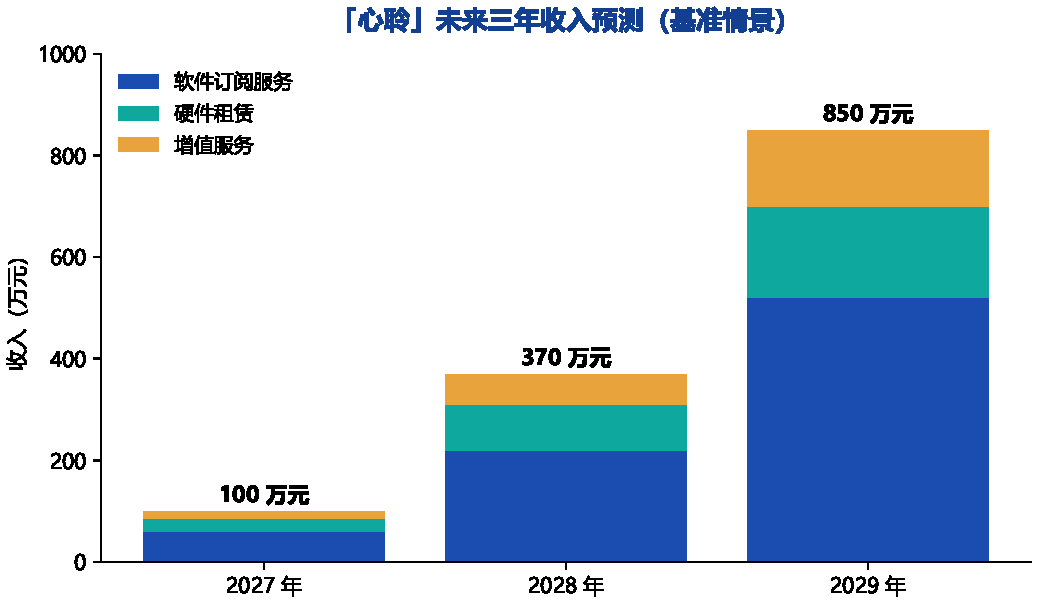
\includegraphics[width=0.72\textwidth]{fig_revenue.pdf}
\caption{“心聆”未来三年收入预测（基准情景）}
\label{fig:revenue}
\end{figure}

收入预测明细如表~\ref{tab:revenue} 所示。

\begin{table}[H]
\centering
\caption{未来三年收入预测明细（单位：万元）}
\label{tab:revenue}
\begin{tabular}{lccc}
\toprule
\textbf{收入项} & \textbf{第一年} & \textbf{第二年} & \textbf{第三年} \\
\midrule
软件订阅 & 60 & 220 & 520 \\
硬件租赁 & 25 & 90 & 180 \\
增值服务 & 15 & 60 & 150 \\
\midrule
合计 & 100 & 370 & 850 \\
\bottomrule
\end{tabular}
\end{table}

\subsection{融资需求与资金用途}

项目计划进行天使轮融资三百万元，出让百分之十股权，资金用途如表~\ref{tab:fund} 所示。

\begin{table}[H]
\centering
\caption{天使轮融资资金用途}
\label{tab:fund}
\begin{tabular}{lcc}
\toprule
\textbf{用途} & \textbf{金额（万元）} & \textbf{占比} \\
\midrule
算法与产品研发 & 150 & 50.0\% \\
硬件量产与备货 & 60 & 20.0\% \\
试点推广与市场 & 60 & 20.0\% \\
资质合规与运营 & 30 & 10.0\% \\
\midrule
合计 & 300 & 100.0\% \\
\bottomrule
\end{tabular}
\end{table}

\subsection{盈亏平衡分析}

以软件订阅为主要收入，盈亏平衡点可由下式近似计算：
\begin{equation}
Q^{*} = \frac{F}{p-v},
\label{eq:breakeven}
\end{equation}
其中 $F$ 为年固定成本，$p$ 为单校年均服务价格，$v$ 为单校可变成本。按年固定成本一百五十万元、单校年均价格三万元、单校可变成本零点八万元测算，盈亏平衡对应约六十八所订阅学校，项目预计于第二年达成。

% ============================================================
% 八、团队介绍
% ============================================================
\section{团队介绍}

\subsection{组织架构}

团队按照“产品研发—市场运营—合规管理”三条线设置岗位，核心岗位如表~\ref{tab:team} 所示。

\begin{table}[H]
\centering
\caption{核心团队组织架构}
\label{tab:team}
\begin{tabular}{p{3.4cm}p{4.4cm}p{5.6cm}}
\toprule
\textbf{岗位} & \textbf{职责} & \textbf{能力要求} \\
\midrule
项目负责人 & 总体统筹、对外联络、资源整合 & 创新创业竞赛经验，项目管理能力 \\
算法负责人 & 特征提取、模型训练与验证 & 脑电信号处理、深度学习、联邦学习 \\
硬件负责人 & 设备选型、联调与量产对接 & 嵌入式软硬件、可穿戴设备经验 \\
产品负责人 & 需求分析、原型设计与交互 & 教育场景理解、产品设计能力 \\
市场负责人 & 客户调研、渠道开拓与路演 & 市场分析、商务谈判能力 \\
合规顾问 & 伦理审查、数据安全与法律合规 & 医学伦理、个人信息保护法 \\
\bottomrule
\end{tabular}
\end{table}

\subsection{核心成员与顾问}

核心成员由电子信息、人工智能、心理学与工商管理等多专业学生组成，形成“技术＋场景＋商业”的互补结构。项目拟聘请心理学院教授担任心理学顾问、临床心理师担任专业顾问、创业导师担任商业顾问，构建产学研协同的支持体系。（团队详细信息以实际成员为准。）

% ============================================================
% 九、风险管理与应对
% ============================================================
\section{风险管理与应对}

\subsection{风险识别与评估}

项目风险识别与评估如表~\ref{tab:risk} 所示。

\begin{table}[H]
\centering
\caption{风险识别与评估矩阵}
\label{tab:risk}
\begin{tabular}{p{2.6cm}p{3.6cm}p{1.8cm}p{5.4cm}}
\toprule
\textbf{风险类型} & \textbf{主要表现} & \textbf{等级} & \textbf{应对措施} \\
\midrule
技术风险 & 跨被试准确率不足、设备噪声大 & 高 & 多数据集验证、域自适应、设备选型测试 \\
数据风险 & 标注数据不足、样本偏差 & 高 & 联邦学习、数据增强、合作医院数据 \\
政策风险 & 伦理与监管趋严、非医疗定位模糊 & 中 & 伦理前置审查、明确定位、动态跟踪政策 \\
隐私风险 & 脑电数据泄露、知情同意缺失 & 高 & 本地化部署、加密存储、最小必要原则 \\
市场风险 & 客户采购周期长、竞品低价竞争 & 中 & 标杆试点、教育局入围、差异化定价 \\
财务风险 & 研发投入大、回款周期长 & 中 & 分期订阅、预收款模式、控制现金消耗 \\
\bottomrule
\end{tabular}
\end{table}

\subsection{伦理与合规设计}

平台遵循“最小必要、知情同意、本地优先、人工复核”四大原则：采集前由学校与监护人完成知情同意；仅采集完成任务所需的最少通道与时段数据；默认数据不出校，梯度更新前完成加密与匿名化；所有高风险结论必须经持证心理教师复核后方可告知家长。项目将同步完成校级伦理审查、个人信息保护影响评估与神经数据安全管理制度的建设，确保在合规框架内开展试点。

% ============================================================
% 十、社会价值与发展规划
% ============================================================
\section{社会价值与发展规划}

\subsection{社会价值}

项目的社会价值体现在四个方面：一是直接提升青少年心理问题发现率，将干预窗口前移，降低心理危机事件发生率；二是为乡村与欠发达地区学校提供低成本的普惠筛查工具，缓解优质心理服务资源不均衡问题；三是带动脑机接口、人工智能与心理健康交叉领域的高质量就业；四是以可复制、可推广的模式服务更多学校，形成“筛查—预警—干预—追踪”的社会治理样本。

\subsection{三年发展规划}

项目发展路线如图~\ref{fig:roadmap} 所示：第一年完成原型开发、伦理审查与五十所试点学校验证；第二年完成产品迭代与三百所学校规模化落地，同步开展医院心理科试点；第三年拓展企业员工关怀场景并探索国际市场。

\begin{figure}[H]
\centering
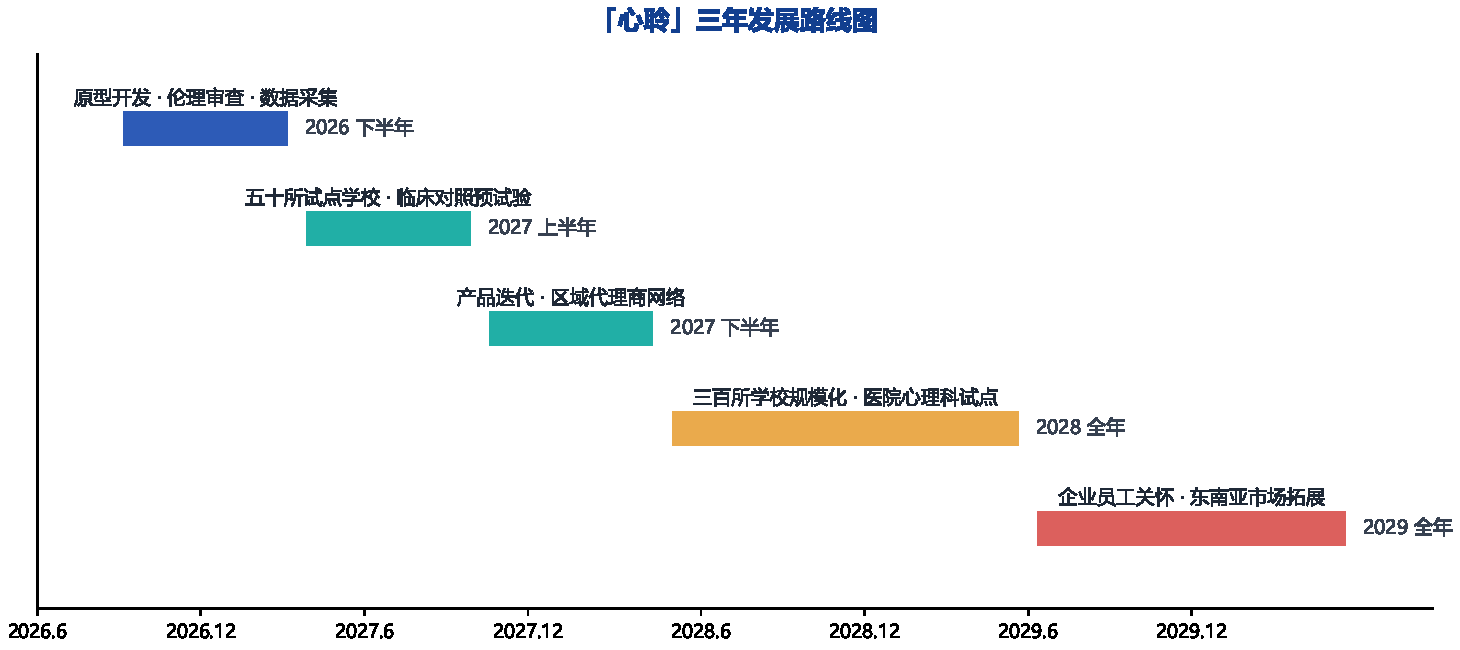
\includegraphics[width=0.95\textwidth]{fig_roadmap.pdf}
\caption{“心聆”三年发展路线图}
\label{fig:roadmap}
\end{figure}

\subsection{项目真实性与可持续性}

项目技术路线源于团队成员在脑电情绪识别方向的研究积累，涉及差分熵特征、图卷积与 Transformer 等方法的复现与改进，具有明确的科学依据；商业计划中的市场数据均标注来源，财务预测基于可检验假设并随试点数据滚动修正；产品坚持“客观筛查、专业复核、非医疗诊断”的边界，确保技术应用在伦理与法律框架内可持续运行。

% ============================================================
% 参考文献
% ============================================================
\begin{thebibliography}{99}

\bibitem{ref1} 教育部, 国家发展改革委, 等. 全面加强和改进新时代学生心理健康工作专项行动计划（2023—2025年）[Z]. 北京: 教育部, 2023.

\bibitem{ref2} 傅小兰, 张侃, 陈雪峰, 等. 中国国民心理健康发展报告（2021—2022）[M]. 北京: 社会科学文献出版社, 2023.

\bibitem{ref3} 教育部办公厅. 进一步加强中小学生心理健康工作十条措施[Z]. 北京: 教育部办公厅, 2025.

\bibitem{ref4} Zheng W L, Lu B L. Investigating critical frequency bands and channels for EEG-based emotion recognition with deep neural networks[J]. IEEE Transactions on Autonomous Mental Development, 2015, 7(3): 162-175.

\bibitem{ref5} Koelstra S, Muhl C, Soleymani M, et al. DEAP: a database for emotion analysis using physiological signals[J]. IEEE Transactions on Affective Computing, 2012, 3(1): 18-31.

\bibitem{ref6} Vaswani A, Shazeer N, Parmar N, et al. Attention is all you need[C]//Advances in Neural Information Processing Systems 30. Long Beach: Curran Associates, 2017: 5998-6008.

\bibitem{ref7} Duan R N, Zhu J Y, Lu B L. Differential entropy feature for EEG-based emotion classification[C]//International IEEE/EMBS Conference on Neural Engineering. San Diego: IEEE, 2013: 81-84.

\bibitem{ref8} Song T, Zheng W, Song P, et al. EEG emotion recognition using dynamical graph convolutional neural networks[J]. IEEE Transactions on Affective Computing, 2020, 11(3): 532-541.

\bibitem{ref9} McMahan B, Moore E, Ramage D, et al. Communication-efficient learning of deep networks from decentralized data[C]//Proceedings of the 20th International Conference on Artificial Intelligence and Statistics. Fort Lauderdale: PMLR, 2017: 1273-1282.

\bibitem{ref10} Lundberg S M, Lee S I. A unified approach to interpreting model predictions[C]//Advances in Neural Information Processing Systems 30. Long Beach: Curran Associates, 2017: 4765-4774.

\bibitem{ref11} 科学技术部. 涉及人的神经技术医学研究伦理指引[R]. 北京: 科学技术部, 2025.

\bibitem{ref12} 观研报告网. 中国心理健康服务行业发展趋势分析与未来投资研究报告（2026—2033年）[R/OL]. (2026-06)[2026-08-12]. https://www.chinabaogao.com/baogao/202606/801069.html.

\bibitem{ref13} 国家卫生健康委员会. 我国儿童青少年心理健康服务体系建设取得重要进展[EB/OL]. (2026-06)[2026-08-12]. https://news.jnyuhope.net/2432.html.

\bibitem{ref14} 全国大学生创业服务网. 中国国际大学生创新大赛（2026）[EB/OL]. (2026)[2026-08-12]. https://cy.ncss.cn.

\end{thebibliography}

% ============================================================
% 附录
% ============================================================
\newpage
\appendix
\renewcommand{\thesection}{附录\Alph{section}}
\ctexset{section={number=\thesection}}
\section{核心算法伪代码}

\subsection{预处理与特征提取伪代码}

\begin{lstlisting}[language=Python,caption=EEG preprocessing and feature extraction]
def extract_features(raw, fs=250):
    # 1. band-pass filter 0.5-45 Hz
    eeg = butter_bandpass(raw, 0.5, 45, fs)
    # 2. remove ocular artifacts via ICA
    eeg = ica_remove(eeg, reject=['EOG'])
    # 3. segment into windows (4 s, 50% overlap)
    windows = sliding_windows(eeg, win=4*fs, step=2*fs)
    feats = []
    for w in windows:
        de = differential_entropy(w)   # Eq.(1)
        psd = welch_psd(w, fs)         # Eq.(2)
        feats.append(concat(de, psd))
    return zscore(feats)               # Eq.(3)
\end{lstlisting}

\subsection{跨被试训练伪代码}

\begin{lstlisting}[language=Python,caption=Cross-subject adversarial training]
for epoch in range(epochs):
    for x, y, sub in loader:
        feat = feature_extractor(x)          # theta_f
        y_hat = classifier(feat)             # theta_c
        sub_hat = domain_discriminator(grl(feat))  # theta_d, GRL
        loss = CE_weighted(y_hat, y) - lam * BCE(sub_hat, sub)
        optimizer.zero_grad(); loss.backward(); optimizer.step()
\end{lstlisting}

\subsection{联邦学习聚合伪代码}

\begin{lstlisting}[language=Python,caption=Federated averaging]
def federated_round(server, schools):
    for school in schools:
        model = server.distribute()
        grads = school.local_update(model, encrypted=True)
        server.aggregate(grads)              # Eq.(7)
\end{lstlisting}

\section{核心公式推导说明}

式(\ref{eq:de}) 的差分熵定义源于香农熵在连续分布下的推广。对于零均值高斯分布 $p(x)=\frac{1}{\sqrt{2\pi\sigma^2}}\exp(-\frac{x^2}{2\sigma^2})$，其熵为
\begin{equation}
h(X)=-\int p(x)\log_2 p(x)\,\mathrm{d}x
=\frac{1}{2}\log_2\left(2\pi\mathrm{e}\sigma^2\right),
\label{eq:de_derive}
\end{equation}
对每个频段分别估计方差后代入即得式(\ref{eq:de})。

式(\ref{eq:psd}) 中 Welch 谱估计通过分段加窗与平均降低方差，$U=\frac{1}{M}\sum_n w^2(n)$ 保证谱估计的渐近无偏性，是脑电节律能量分析的标准方法。

\section{术语表}

\begin{tabular}{p{3.2cm}p{10.6cm}}
\toprule
\textbf{术语} & \textbf{说明} \\
\midrule
差分熵 & 描述信号不确定性的信息论特征，与脑电节律能量相关 \\
效价与唤醒度 & 情绪维度模型的两个主轴，分别刻画愉悦程度与激活程度 \\
跨被试泛化 & 模型在未见过的个体上的识别能力 \\
联邦学习 & 数据不出本地、仅共享模型更新的分布式训练范式 \\
梯度反转层 & 通过反转梯度使特征对被试身份不敏感的技术 \\
SHAP 值 & 基于博弈论的模型特征贡献解释方法 \\
\bottomrule
\end{tabular}

\section{支撑材料清单}

\begin{enumerate}
  \item 项目 LOGO 设计源文件（PNG 与 SVG）；
  \item 公开数据集复现实验记录（SEED、DEAP）；
  \item 情绪诱发任务素材清单与伦理审查申请材料；
  \item 竞品调研与行业报告整理文档；
  \item 财务预测模型（可编辑表格）。
\end{enumerate}

\end{document}
